\documentclass{article}
\usepackage[utf8]{inputenc}
\usepackage{graphicx}
\usepackage{geometry}
\usepackage{hyperref}

\title{Testing policy Document}
\author{TeamTuring:\\\\Darius Scheepers, Kyle Pretorius, Richard Dixie, Sewis van Wyk,\\\\ Tristan Rothman \& Ulrik de Muelenaere\\\\ ERP-Coin}
\date{}

\begin{document}
\maketitle
\begin{center}

\includegraphics[scale=0.1]{erp-logo.png}
\end{center}

\begin{center}

\includegraphics[scale=0.15]{epi-use.png}
\end{center}

\section{Testing process}
We have a policy that feature branches may only be merged into the main development branch if all tests pass, and similarly for merging the development branch into master. This is enforced by Travis CI, which automatically runs tests on each pull request.
\\ \\
\subsection*{Functional requirements tests}
Our back end is based on the Node.js framework and for this reason will be tested using Mocha. Due to the nature of our system, all requests will run through the central server, which allows us to create a central point of testing. All use cases can be expressed in terms of requests that must be sent to the server, hence our tests will be request-based and can be divided into modules that are formed by the APIs provided by our server.
\\ \\
As stated above, any changes made to the server will be extensively tested before they are merged with the main branch. The smallest units of the server can be seen as features, hence we will perform unit tests on each feature to ensure that it works as intended before merging it into the main development branch. The features will be tested again as part of the larger system in the development branch as part of integration testing. Once these tests pass as well, then only may the development branch be merged into the main branch and testing may start again on new features.
\\ \\
\subsection*{Non-functional requirements test}

\begin{itemize}
\item Security: \\
These tests are focused on the requirement that no unauthorized user may have access to the system. The system achieves this by testing that a user is logged in with every request. This creates the following two possible outcomes:
\begin{enumerate}
    \item The user is logged in, and their request may be processed.
    \item The user is not logged in, and the request must be rejected.
\end{enumerate}

\item Validation:\\
This testing focuses that our system will correctly accept requests that contain valid data and will reject requests that contain invalid data. This prevents our system from entering an invalid state or storing invalid information on the database. 

\item Correctness:\\
These tests focus on ensuring that the server performs as expected when a request to is made by a user. This includes testing that data is actually inserted into the database when a request is made, such as adding a new user or logging points where users have been. Another correctness test performed is to ensure that data returned by the server to the ERP Coin mobile application is valid.
\\ \\
\end{itemize}

\section{Testing tools}
For this project the main testing tool used is Mocha, which is a JavaScript testing framework running on Node.js. This framework allows us to extensively test our back end, which is our system's main point of computation through which all use cases run. The server runs on Node.js, making Mocha ideal for testing its functionality. We use SuperTest in conjunction with Mocha, since most of our tests take the form of HTTP requests. SuperTest is a tool to simulate HTTP requests in unit tests.
\\\\
Our Ethereum smart contracts are created using the Truffle framework. This framework also integrates with Mocha, which we use to test the methods provided by our smart contract. It is particularly important to test the smart contract, since it is stored immutably on the blockchain, so mistakes cannot be fixed once the contract is deployed.
\\\\
To improve code quality, ESLint is used for ensuring that the code conforms to the coding conventions for the project. JavaScript, being a dynamic and loosely-typed language, is especially prone to developer error. Without the benefit of a compilation process, JavaScript code is typically executed in order to find syntax or other errors. Linting tools like ESLint allow developers to discover problems with their JavaScript code without executing it. ESLint is configured by use of a \texttt{.eslintrc.json} file. The configuration file used for this project can be found here: \url{https://github.com/TeamTuringCOS301/back-end/blob/master/.eslintrc.json}
\\\\
Since the user interfaces are written in TypeScript, we use TSLint instead of ESLint in these repositories.
\\\\
Finally, we use Travis CI to automatically run these tests on all pull requests. This allows us to enforce the policy that branches may not be merged if the tests do not pass.
\\\\
The tools we use can be found at the following locations:
\begin{itemize}
\item Mocha: \url{https://mochajs.org/}
\item SuperTest: \url{https://github.com/visionmedia/supertest}
\item Truffle: \url{https://truffleframework.com/}
\item ESLint: \url{https://eslint.org/}
\item TSLint: \url{https://palantir.github.io/tslint/}
\item Travis CI: \url{https://travis-ci.org/}
\end{itemize}

\newpage
\section{Test cases}
The tests for the HTTP API are in the following directory:\\
\url{https://github.com/TeamTuringCOS301/back-end/tree/master/test}
\\\\
This directory contains the following files:
\begin{itemize}
\item \texttt{mock-config.js}, \texttt{mock-db.js}, \texttt{mock-coins.js}, \texttt{mock-email.js}: These files mock the interfaces provided by the configuration file, database, Ethereum blockchain and SMTP server, respectively. This allows us to write tests that do not depend on these external services.
\end{itemize}
The rest of the files each test the HTTP API for one of our subsystems:
\begin{itemize}
\item \texttt{user-api.js}: This tests the user API, which is responsible for user management. It provides routes for users to create accounts, log in and out, and update their account details. It also keeps track of the number of coins earned by each user.
\item \texttt{superadmin-api.js}: This tests the API provided for the main admin users. These users can add new conservation areas and conservation area admins.
\item \texttt{admin-api.js}: This tests the API provided for conservation area admins. These admins can view alerts posted in their assigned areas, and suggest rewards to be made available to users.
\item \texttt{area-api.js}: This tests the conservation area API. It provides routes to add and remove conservation areas, update the information of conservation areas, and keep track of the conservation area border.
\item \texttt{point-api.js}: This tests the point API. It allows users to record their position within the conservation area border, and aggregates the points so that users can see which areas have been visited most frequently.
\end{itemize}
To run the tests described above, execute the command \texttt{npm test}.
\\\\
The unit tests for the Ethereum smart contract can be found in the follwoing file:\\
\url{https://github.com/TeamTuringCOS301/back-end/tree/master/token/test/erp-coin.js}\\
To run these tests, execute the command \texttt{npm run truffle test}.

\section{History}
The full test logs can be found on the Travis CI website:\\
\url{https://travis-ci.org/TeamTuringCOS301/back-end}\\
Below are some excerpts from the latest test log.
\\\\
The first excerpt shows that ESLint was run successfully, without producing any warnings:\\
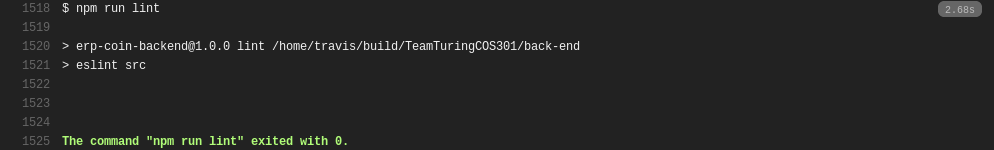
\includegraphics[scale=0.43]{eslint-log.png}
\\\\
The next excerpt shows the tests for one of the HTTP APIs, in particular the conservation area admin API. This includes both functional and non-functional tests:
\begin{itemize}
\item Lines 1538--1540, 1548, 1556, 1562, 1565, 1569 and 1573 are functional tests.
\item Lines 1535, 1542, 1547, 1551, 1554, 1559, 1561, 1568 and 1571 are security tests.
\item Lines 1536, 1537, 1543, 1545, 1546, 1555, 1560 and 1572 are validation tests.
\item Lines 1541, 1549, 1552, 1557, 1563, 1566 and 1574 are correctness tests.
\end{itemize}
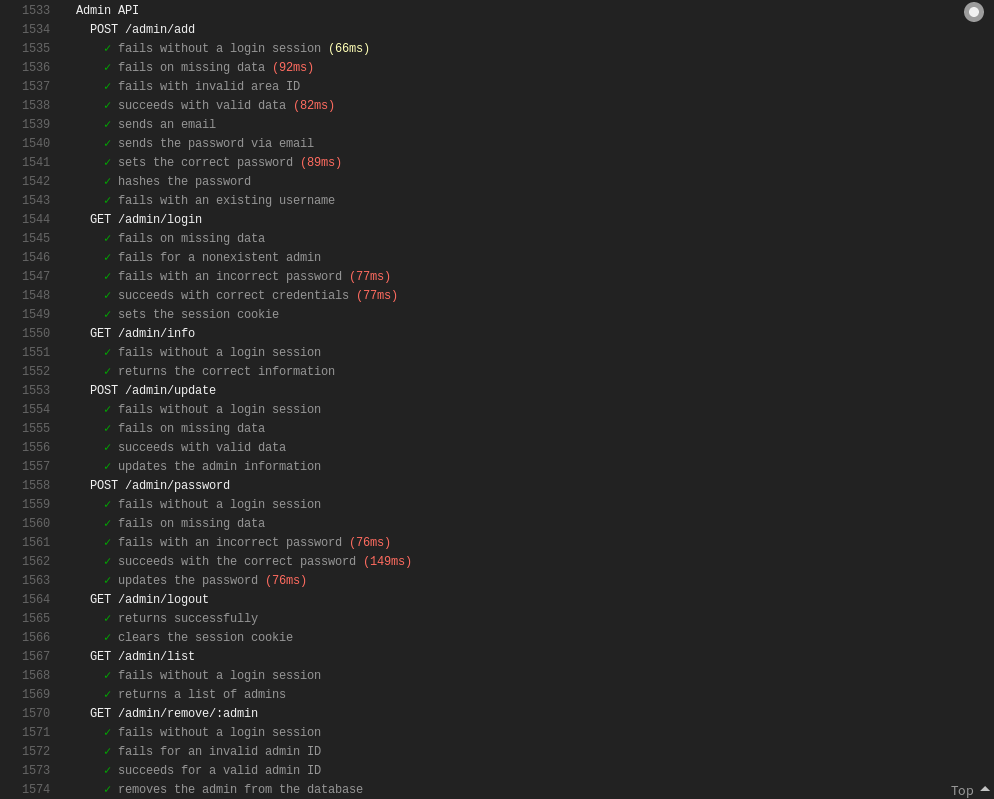
\includegraphics[scale=0.43]{admin-api-log.png}
\newpage
\noindent The final excerpt contains the results of the smart contract tests. As above, this includes both functional and non-functional tests.\\
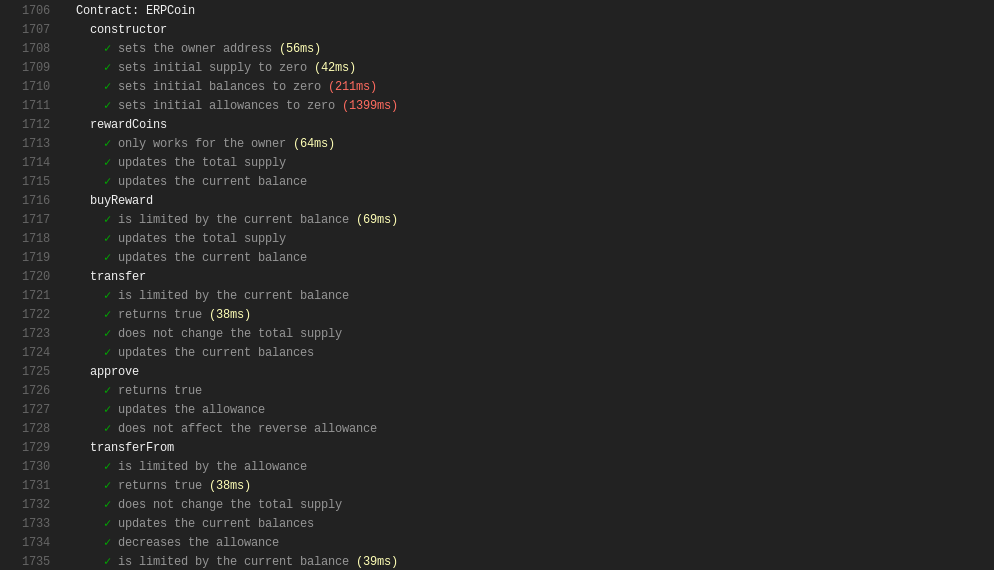
\includegraphics[scale=0.43]{contract-log.png}

\end{document}
